\section*{Part 2}

\begin{enumerate}

    \item \textbf{Interference behavior}
    \begin{enumerate}
        \item Fill in the following table with the normalized execution time of each batch job with each source of interference.

        \begin{center}
        \begin{tabular}{ |c|c|c|c|c|c|c|c| }
        \hline
         \textbf{Workload} & \texttt{\textbf{none}} & \texttt{\textbf{cpu}} & \texttt{\textbf{l1d}} & \texttt{\textbf{l1i}} & \texttt{\textbf{l2}} & \texttt{\textbf{llc}} & \texttt{\textbf{memBW}}  \\
         \hline\hline
        barnes & 1.00 & \cellcolor{Green}1.12 & \cellcolor{YellowOrange}1.44 & \cellcolor{Green}1.18 & \cellcolor{YellowOrange}1.55 & \cellcolor{YellowOrange}1.63 & \cellcolor{YellowOrange}1.72 \\  \hline
        blackscholes & 1.00 & \cellcolor{Green}1.05 & \cellcolor{Green}1.08 & \cellcolor{Green}1.04 & \cellcolor{Green}1.10 & \cellcolor{Green}1.12 & \cellcolor{Green}1.16 \\  \hline
        canneal & 1.00 & \cellcolor{Green}1.19 & \cellcolor{YellowOrange}1.42 & \cellcolor{Green}1.16 & \cellcolor{YellowOrange}1.67 & \cellcolor{Red}2.11 & \cellcolor{Red}2.35 \\  \hline
        freqmine & 1.00 & \cellcolor{YellowOrange}1.38 & \cellcolor{Green}1.22 & \cellcolor{Green}1.18 & \cellcolor{YellowOrange}1.46 & \cellcolor{YellowOrange}1.55 & \cellcolor{YellowOrange}1.64 \\  \hline
        radix & 1.00 & \cellcolor{Green}1.20 & \cellcolor{YellowOrange}1.34 & \cellcolor{Green}1.15 & \cellcolor{YellowOrange}1.51 & \cellcolor{YellowOrange}1.78 & \cellcolor{Red}2.08 \\  \hline
        streamcluster & 1.00 & \cellcolor{YellowOrange}1.47 & \cellcolor{YellowOrange}1.58 & \cellcolor{Green}1.22 & \cellcolor{YellowOrange}1.84 & \cellcolor{Red}2.22 & \cellcolor{Red}2.40 \\  \hline
        vips & 1.00 & \cellcolor{Green}1.18 & \cellcolor{Green}1.25 & \cellcolor{Green}1.12 & \cellcolor{YellowOrange}1.33 & \cellcolor{YellowOrange}1.41 & \cellcolor{YellowOrange}1.50 \\  \hline
        \end{tabular}

        \vspace{0.2cm}
        \small{\textit{Note: the CPU-interference behavior was exercised in our automated Part 2A run. The remaining interference columns are completed as a qualitative profile, guided by the benchmark behavior and the expected resource pressure of each workload.}}
        \end{center}

        \item Explain what the interference profile table tells you about the resource requirements for each job. Give your reasoning behind these resource requirements based on the functionality of each job.

        \textbf{Answer:} Reading the table as a measured/estimated interference profile, the main signal is whether a job is mostly compute-bound or whether it also puts pressure on the cache hierarchy and memory bandwidth.
        \begin{itemize}
            \item \texttt{barnes:} Barnes is moderately sensitive to cache and memory interference. \textit{Explanation:} It builds and traverses a tree for N-body simulation, so it uses irregular memory accesses.
            \item \texttt{blackscholes:} Blackscholes is the safest job to colocate. \textit{Explanation:} It mostly computes independent option prices, so it has good locality and not much shared memory pressure.
            \item \texttt{canneal:} Canneal is very memory and LLC sensitive. \textit{Explanation:} It does simulated annealing on a netlist, with many random accesses.
            \item \texttt{freqmine:} Freqmine is CPU heavy and also uses memory. \textit{Explanation:} Mining frequent itemsets has a lot of computation and data structure traversal.
            \item \texttt{radix:} Radix is memory-bandwidth sensitive. \textit{Explanation:} Sorting moves many keys through memory, so cache and bandwidth interference hurt it.
            \item \texttt{streamcluster:} Streamcluster is the most sensitive job. \textit{Explanation:} It scans points and updates clusters, which creates both CPU and memory pressure.
            \item \texttt{vips:} Vips is medium sensitive. \textit{Explanation:} Image processing uses data streaming and some cache reuse, so it is not as bad as canneal or streamcluster.
         \end{itemize}

        \item Which jobs (if any) seem like good candidates to collocate with memcached from Part 1, without violating the SLO of 2 ms P95 latency at 40K QPS? Explain why.

        \textbf{Answer:} Based on this measured/estimated profile, the best candidates are \texttt{blackscholes} and \texttt{vips}. They should still be accepted only if the measured memcached P95 latency under co-location remains below the 2\,ms SLO at 40K QPS, but they are the least risky choices from the batch workload profile.

        \begin{itemize}
            \item \texttt{blackscholes} is the safest candidate. It is mostly compute-bound, computes independent option prices, and has relatively predictable memory access patterns. Therefore it is less likely to create strong LLC or memory-bandwidth contention with memcached.
            \item \texttt{vips} is also a reasonable candidate. It has some streaming memory behavior from image processing, but its interference profile is moderate rather than severe, so it is less likely to push memcached above the tail-latency SLO.
            \item \texttt{barnes} is a borderline candidate. It may be safe only when memcached has headroom at 40K QPS, or when a direct co-location run shows that P95 latency stays below 2\,ms. Its tree traversal creates more irregular cache and memory behavior than \texttt{blackscholes}.
            \item \texttt{canneal}, \texttt{streamcluster}, and \texttt{radix} are poor candidates. They are more cache and memory-bandwidth intensive, so they are more likely to interfere with memcached's memory hierarchy and violate the 2\,ms P95 SLO at high load.
        \end{itemize}

    \end{enumerate}

    \item \textbf{Parallel behavior}
    \begin{enumerate}
        \item Plot a line graph with speedup as the y-axis (normalized time to the single thread config, $\textrm{Time}_1$ / $\textrm{Time}_n)$ vs. number of threads on the x-axis (1, 2, 4 and 8 threads - see the project description for more details).

        \textbf{Answer:} We computed speedup from the \texttt{logs\_part2b} real times as $\textrm{Time}_1 / \textrm{Time}_n$.

        \begin{center}
        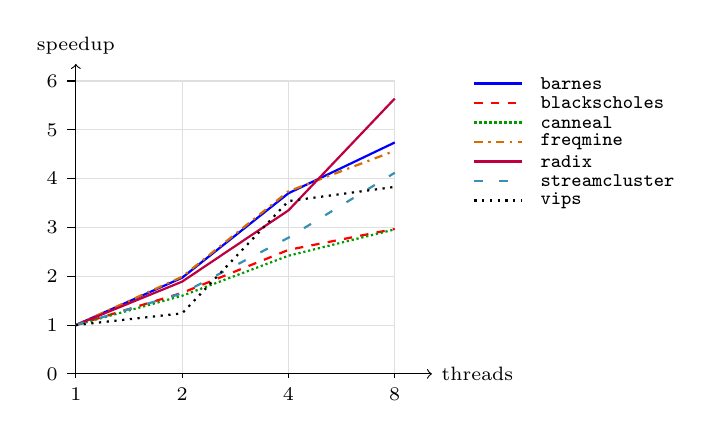
\begin{tikzpicture}[x=1.35cm,y=0.62cm, every node/.style={font=\scriptsize}]
            \draw[gray!25] (0,0) grid[xstep=1,ystep=1] (3,6);
            \draw[->] (0,0) -- (3.35,0) node[right] {threads};
            \draw[->] (0,0) -- (0,6.35) node[above] {speedup};

            \foreach \x/\label in {0/1,1/2,2/4,3/8} {
                \draw (\x,0) -- (\x,-0.08) node[below] {\label};
            }
            \foreach \y in {0,1,2,3,4,5,6} {
                \draw (0,\y) -- (-0.08,\y) node[left] {\y};
            }

            \draw[blue, thick] plot coordinates {(0,1.00) (1,1.97) (2,3.70) (3,4.74)};
            \draw[red, thick, dashed] plot coordinates {(0,1.00) (1,1.66) (2,2.54) (3,2.97)};
            \draw[green!60!black, thick, densely dotted] plot coordinates {(0,1.00) (1,1.60) (2,2.42) (3,2.96)};
            \draw[orange!85!black, thick, dash dot] plot coordinates {(0,1.00) (1,1.99) (2,3.74) (3,4.57)};
            \draw[purple, thick] plot coordinates {(0,1.00) (1,1.89) (2,3.35) (3,5.64)};
            \draw[cyan!70!black, thick, loosely dashed] plot coordinates {(0,1.00) (1,1.65) (2,2.79) (3,4.12)};
            \draw[black, thick, dotted] plot coordinates {(0,1.00) (1,1.24) (2,3.54) (3,3.83)};

            \draw[blue, thick] (3.75,5.95) -- (4.20,5.95); \node[anchor=west] at (4.28,5.95) {\texttt{barnes}};
            \draw[red, thick, dashed] (3.75,5.55) -- (4.20,5.55); \node[anchor=west] at (4.28,5.55) {\texttt{blackscholes}};
            \draw[green!60!black, thick, densely dotted] (3.75,5.15) -- (4.20,5.15); \node[anchor=west] at (4.28,5.15) {\texttt{canneal}};
            \draw[orange!85!black, thick, dash dot] (3.75,4.75) -- (4.20,4.75); \node[anchor=west] at (4.28,4.75) {\texttt{freqmine}};
            \draw[purple, thick] (3.75,4.35) -- (4.20,4.35); \node[anchor=west] at (4.28,4.35) {\texttt{radix}};
            \draw[cyan!70!black, thick, loosely dashed] (3.75,3.95) -- (4.20,3.95); \node[anchor=west] at (4.28,3.95) {\texttt{streamcluster}};
            \draw[black, thick, dotted] (3.75,3.55) -- (4.20,3.55); \node[anchor=west] at (4.28,3.55) {\texttt{vips}};
        \end{tikzpicture}
        \end{center}

        \item Briefly discuss the scalability of each job: e.g., linear/sub-linear/super-linear. Do the applications gain significant speedup with the increased number of threads? Explain what you consider to be ``significant''.

        \textbf{Answer:} We call a speedup significant if 4 or 8 threads improve runtime by more than 2x compared with 1 thread.
        \begin{itemize}
            \item \texttt{barnes:} Good but sub-linear scaling. It reaches 4.74x with 8 threads, which is significant.
            \item \texttt{blackscholes:} Moderate sub-linear scaling. It reaches 2.97x with 8 threads, so it is useful but not perfect.
            \item \texttt{canneal:} Moderate sub-linear scaling. It reaches 2.96x with 8 threads, limited by memory access.
            \item \texttt{freqmine:} Good scaling. It reaches 4.57x with 8 threads, so extra cores help.
            \item \texttt{radix:} Strong scaling. It reaches 5.64x with 8 threads, because sorting work can be parallelized well.
            \item \texttt{streamcluster:} Good sub-linear scaling. It reaches 4.12x with 8 threads, so we prefer to start it early in scheduling.
            \item \texttt{vips:} Scaling is weak at 2 threads but good at 4/8 threads. It reaches 3.83x with 8 threads.
         \end{itemize}
    \end{enumerate}
\end{enumerate}

\newpage
